% Iran's electricity deficit — IEEE format, no page limit.
\documentclass[conference]{IEEEtran}
\usepackage[T1]{fontenc}
\usepackage[utf8]{inputenc}
\usepackage{graphicx}
\usepackage{booktabs}
\usepackage{amsmath}
\usepackage{array}
\setlength{\emergencystretch}{1.5em}

\begin{document}

\title{Iran's Electricity Deficit:\\ Measurement, Trend Projection, and the Scale of the Required Response}

\author{
\IEEEauthorblockN{
Ramtin Ghiyami\IEEEauthorrefmark{1},
Matin Askari\IEEEauthorrefmark{1},
Ali Zafari\IEEEauthorrefmark{1}
}
\IEEEauthorblockA{
\IEEEauthorrefmark{1}
Department of Computer and Data Sciences, Faculty of Mathematical Sciences,\\
Shahid Beheshti University, Tehran, Iran\\
Email: ramtinrgextreme@gmail.com, dev.mtnaskari@gmail.com, a.zafari.110@gmail.com
}
}

\maketitle

\begin{abstract}
Iran's summer blackouts are widely reported, but the size, trajectory and composition of the underlying imbalance are rarely measured from primary records. This paper assembles a 58-year annual panel of the Iranian power system from the industry's own statistical publications --- peak generating capability, maximum supplied load, maximum simultaneous demand, network losses and thermal efficiency, 1346--1403 (1967--2025), extended to 1404 and monthly through 1405-05 from the officially registered workbooks --- validates it across independent documents, and uses it to answer two questions: how large does the peak deficit become if current trends continue, and what scale of response would close it. Defining the peak deficit as maximum simultaneous demand minus maximum supplied load, the deficit was below 2\% of demand as recently as 1398, reached 17.6~GW (21.9\% of demand) in 1403 and 14.9~GW (19.3\%) in 1404. A Welch test on annual growth rates locates the break on the supply side: demand growth before and after 1395 is statistically indistinguishable ($p=0.32$), while the growth of supplied load falls from about 6\% to about 2\% per year ($p=0.035$; $p=0.07$ after a Holm correction across the two tests). Internationally, Iran's generation growth over the last decade (3.5\%/yr) exceeded the world average (2.8\%/yr): the deficit is not a failure to grow in absolute terms but a widening wedge between $\sim$5\%/yr demand growth and $\sim$2\%/yr growth in dependable supply. Extrapolating both trends with a residual bootstrap yields a deficit of 27.8~GW by 1408 (95\% band 22.6--32.9) and 41.5~GW by 1412 (35.3--46.9), or 36\% of projected peak demand. Network losses of 10.3\% --- equivalent to roughly 8~GW at the 1403 peak, more than half of the deficit itself, and concentrated in distribution --- indicate that loss reduction is the cheapest available increment of effective supply. The investment translation of the capacity requirement is stated as an explicit formula whose cost inputs (regulated tariffs, cost of service, guaranteed-purchase rates) are documented as pending. All numbers are computed offline from an identified set of source documents whose provenance is registered file by file.
\end{abstract}

\begin{IEEEkeywords}
electricity deficit, Iran, peak demand, capacity adequacy, network losses, trend projection, residual bootstrap, energy statistics
\end{IEEEkeywords}

\section{Introduction}
Iran entered the 1400s (2020s) with a power system that no longer clears its own summer peak. Rolling blackouts, industrial curtailment quotas and winter gas-for-power shortages are now annual events, and public debate quotes deficit figures ranging from a few gigawatts to more than twenty. What is missing is not attention but measurement: a continuous, source-identified series of how much demand existed, how much was served, and how fast the two have been diverging.

This paper builds that series from the power industry's own statistical record and takes it to the two questions a planner would ask. First, \emph{how large does the deficit become if current trends continue} --- answered with an explicit trend model and an uncertainty band rather than a point guess. Second, \emph{what scale of response closes it} --- answered in physical units (gigawatts of dependable capacity, points of network loss), with the monetary translation stated as a formula whose price inputs are documented as pending rather than filled with unsourced assumptions.

The contribution is fourfold. First, a 58-year annual panel of peak-hour supply and demand (1346--1403), extended to 1404 and monthly into 1405, parsed from the industry's own publications and validated across independent documents. Second, a definition-first measurement of the deficit, with every construction choice stated. Third, statistical evidence on the origin of the imbalance: growth-rate tests locate the break on the supply side, and an international mirror shows Iran's generation growth has not lagged the world --- the wedge is domestic demand growth against dependable-capacity growth. Fourth, a conditional projection with a residual bootstrap, and the explicit arithmetic connecting the projected gap to the scale of the required response.

\section{Data Sources and Provenance}
\label{sec:data}
All primary inputs are official publications of the Iranian power industry, collected manually from the industry's statistics portal (the sources offer no programmatic interface); the analysis stages read only these local files, offline and deterministically. A provenance register lists, for every file, what it is, where it came from and which pipeline stage consumes it.

Four document families carry the analysis. (i) The 58-year statistical retrospective (``58 Years of Iran's Electric Power Industry in the Mirror of Statistics,'' 1346--1403), whose peak-history table reports, per year, the maximum generating capability (grid, off-grid, total), the maximum load actually supplied, the maximum simultaneous demand, the industrial load at the peak hour and the load factor; and whose indicator table reports network losses (total, and the transmission/distribution split where published), thermal-plant efficiency and per-capita quantities over the same 58 years. (ii) The officially registered single-year workbooks (``Official Statistics of the Electric Power Industry,'' 1399--1404), including the two indicators that matter most here: registered peak demand and generating capability at the peak. (iii) The monthly simultaneous-peak sheet, covering every month of 1404 and 1405 through Mordad. (iv) A sectoral sales table (residential, public, industrial, agricultural, street lighting; 1378--1398). Household- and industry-side energy surveys of the Statistical Centre of Iran (1383--1402) are held in the same snapshot for the demand-side extension.

One international series is used as a mirror: country-year electricity generation from the Our World in Data energy compilation (itself built from Ember and the Energy Institute), retained locally so the comparison also runs offline.

Three further official sources exist but sit behind user registration on the industry portal and were not obtainable for this study: the projects pipeline (capacity under construction), the industry's own demand forecast, and the national energy balance. Their absence is treated as a limitation in Section~\ref{sec:limits}, not silently ignored: each would sharpen exactly one section of this paper.

\section{Dataset Construction and Validation}
\label{sec:construction}
The primary tables are published as PDF typography, not as data. Parsing them reliably required two rules learned the hard way and now asserted in code: Arabic presentation-form glyphs must be normalised (NFKC) before any text matching, and a four-digit number in the 1300--1500 range is a year label only at the start of a row --- megawatt and kilowatt-hour values routinely pass through that range and must not be tokenised as years. Each parser ends in loud assertions (year coverage complete, magnitudes in range, known anchor values matched) and the pipeline is bit-reproducible: rerunning every stage reproduces every output byte-for-byte.

Validation follows the same principle as our earlier work on Iranian inflation: agreement between documents with no common typesetting path. Three cross-checks came out exact. The 1403 registered peak in the single-year workbook (79{,}872~MW, grid basis) differs from the 58-year table's figure (80{,}065~MW, whole-country basis) by 193~MW --- almost exactly the published off-grid capability (194~MW), confirming that the two documents measure the same event on stated bases. The maximum of the monthly-peak sheet for 1404 (77{,}497~MW) matches the registered annual figure (77{,}498~MW) to 1~MW. And total network losses for 1403 appear as 10.32\% in both the indicator table and the workbook, to the last digit.

The audit also found an error, which we report rather than suppress: the 58-year table's ``industrial load at peak'' for 1401 reads 31{,}193~MW, roughly ten times its neighbours; the interquartile-range rule flags it as the series' only outlier, and inspection of the typography indicates a footnote marker fused to a value of $\sim$3{,}119~MW. The column is not used in any model; the correction is noted for users of the source.

\section{The Deficit: Definition and Measurement}
\label{sec:deficit}
Everything in this paper hangs on one definition, so it is stated once and used everywhere:
\begin{equation}
\text{peak deficit (MW)} \;=\; D_{\max} - S_{\max},
\end{equation}
where $D_{\max}$ is the maximum simultaneous demand --- the industry's own estimate, which includes load it curtailed --- and $S_{\max}$ is the maximum load actually supplied. The deficit is therefore the demand that existed and was not served at the annual peak: the operational face of the imbalance. The deficit share is the same quantity as a fraction of $D_{\max}$. For 1404, where the 58-year table does not yet reach, both terms come from the registered workbook on the grid basis; Section~\ref{sec:construction} showed the bases agree to about a quarter of one per cent.

\begin{figure}[t]
\centering
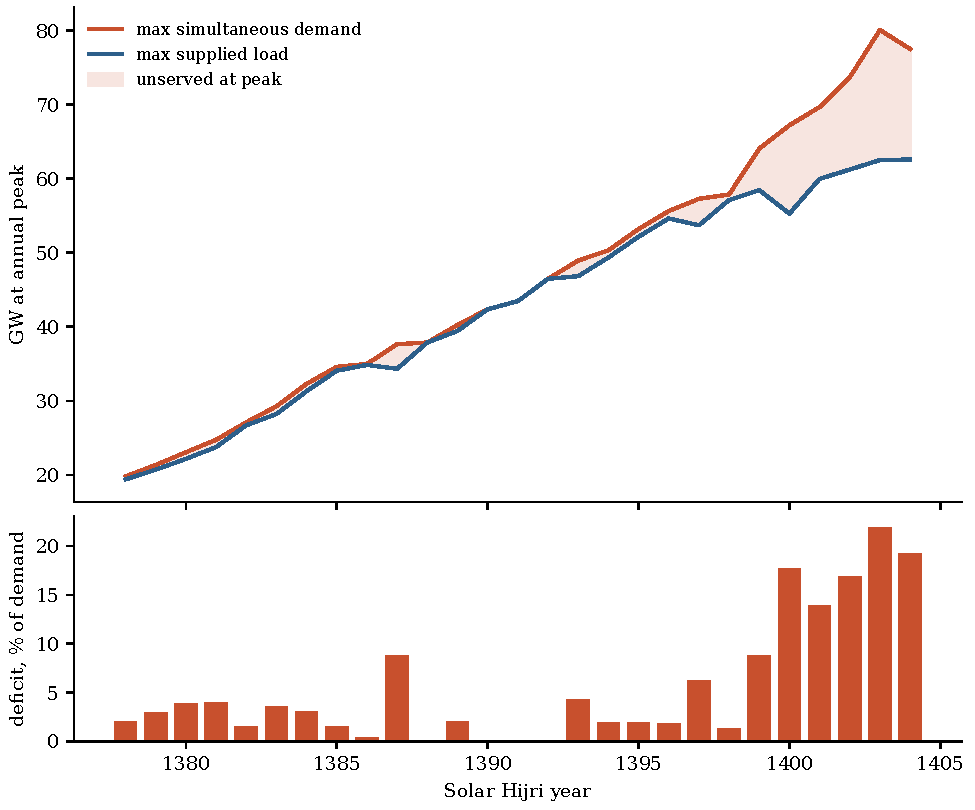
\includegraphics[width=\columnwidth]{figures/fig_deficit_history.pdf}
\caption{Annual peak: maximum simultaneous demand vs.\ maximum supplied load (top) and the deficit as a share of demand (bottom), 1378--1404. The two lines separate from 1399.}
\label{fig:deficit}
\end{figure}

Fig.~\ref{fig:deficit} shows the result. Iran has run episodic peak shortfalls before --- the war years and the early 1370s both show gaps --- but through 1377--1398 the system essentially cleared its peak: the deficit share exceeds 5\% only once in that window. The current episode is different in level and persistence: from below 2\% in 1398 the share rises to 8.8\% in 1399, 17.7\% in 1400, and has remained between 14\% and 22\% since. In 1403 demand of 80.1~GW met supply of 62.5~GW, a deficit of \textbf{17.6~GW (21.9\%)}; in 1404, 77.5~GW of registered demand met 62.6~GW of capability at peak, a deficit of \textbf{14.9~GW (19.3\%)}. The monthly sheet shows the seasonal anatomy: the 1404 peak (77{,}497~MW, 7~Mordad) is 68\% above the winter minimum, and 1405's monthly peaks track 1404's within a few per cent through Mordad.

\section{Where the Deficit Came From: a Supply-Side Break}
\label{sec:break}
Two competing narratives could explain Fig.~\ref{fig:deficit}: demand accelerated, or supply stalled. The growth rates decide. Over 1395--1403 maximum demand grew at 5.2\%/yr while maximum supplied load grew at 2.3\%/yr; the wedge of roughly three percentage points per year, compounded, is the deficit.

To test which side changed, annual growth rates of each series were compared before and after 1395 with a two-sample Welch test. Demand growth averaged 5.9\%/yr through 1395 and 4.3\%/yr after --- a difference the test cannot distinguish from zero ($t=1.03$, $p=0.324$): demand has simply continued its long-run path. Supplied-load growth, by contrast, fell from 6.0\%/yr to 2.1\%/yr ($t=2.31$, $p=0.035$). Because two tests are run at once, we also report Holm-adjusted values: $p=0.32$ for demand and $p=0.07$ for supply --- the supply break is significant at the 10\% level but not at 5\% once the correction is applied, and we state it so. The identification does not rest on the test alone: the deficit itself and the growth-rate wedge of Section~
ef{sec:deficit} are observed quantities, and the test only asks which side moved. A Diebold--Mariano comparison of forecast accuracy, standard in our earlier work, is not applicable here: the projection horizon has not yet occurred, and a backtest would offer roughly five annual points, far too few for the test to carry power. The deficit is a supply-side phenomenon; demand is the backdrop, not the shock.

The international mirror sharpens the point. Over 2014--2024 Iran's electricity generation grew at 3.5\%/yr against a world average of 2.8\%/yr, and Iran's per-capita generation ($\sim$4{,}280~kWh) stands above the world mean ($\sim$3{,}860~kWh). Iran has not stopped building in absolute terms; what it has stopped doing is expanding \emph{dependable peak capability} at the pace of its own demand. The gap between 3.5\%/yr energy growth and 2\%/yr peak-capability growth is itself informative: an ageing thermal fleet, hydro variability and fuel constraints erode the megawatts available at the moment they are needed, even as annual energy output rises.

\section{Network Losses: the Cheapest Unbuilt Power Plant}
\label{sec:losses}
Total network losses fell from a peak near 20\% in the mid-1380s to 10.3\% in 1403 --- a genuine engineering achievement, and one of the few improving series in the record. Even so, 10.3\% of an 80-GW peak is roughly \textbf{8~GW}: more than half of the current deficit is dissipated between the busbar and the meter. The split identifies where: 9.6 points of the 10.3 are lost in distribution against 2.9 in transmission and sub-transmission (the two components overlap in base and do not sum to the total). Every point of distribution loss recovered is worth about 0.8~GW at the current peak --- capacity that requires no fuel, no water and no new right-of-way. Any costed response to the deficit should therefore price loss reduction alongside new build; Section~\ref{sec:budget} carries this explicitly.

\section{Trend Projection with an Uncertainty Band}
\label{sec:projection}
The projection answers a deliberately narrow question: \emph{if the observed trajectories continue, how large is the gap?} Peak demand is fitted with a log-linear trend on 1390--1404 (fifteen points spanning pre- and post-deficit years; fitted growth 4.7\%/yr) and maximum supplied load on 1395--1404 (the capacity-constrained era; fitted growth 2.0\%/yr --- a longer window would import a growth rate the system no longer achieves). Both trends are extended to 1412, and the deficit is their difference. Uncertainty is quantified by resampling each fit's residuals i.i.d.\ 4{,}000 times around the trend paths with a fixed seed; the 95\% band on the deficit combines both draws. This treats the trend as fixed and randomises around it --- a residual bootstrap, honest about being a conditional extrapolation rather than a structural model: it is not a forecast of policy, weather or war.

\begin{figure}[t]
\centering
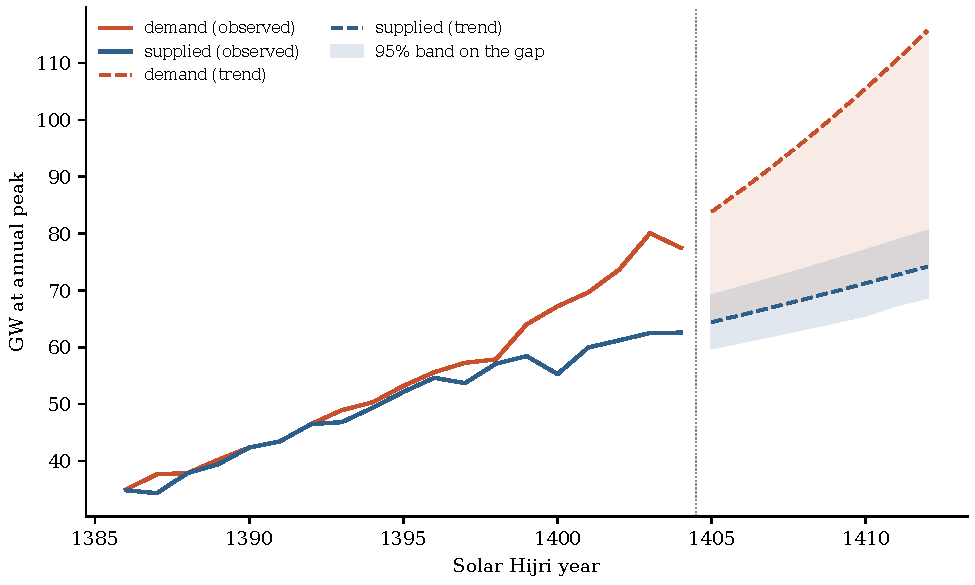
\includegraphics[width=\columnwidth]{figures/fig_deficit_forecast.pdf}
\caption{Observed and projected annual peak, with the 95\% bootstrap band on the projected gap. Dashed lines extend the fitted trends; the dotted vertical marks the last observed year (1404).}
\label{fig:forecast}
\end{figure}

\begin{table}[t]
\caption{Projected peak deficit under current trends (GW). Band: 2.5th--97.5th percentile of the residual bootstrap.}
\label{tab:forecast}
\centering
\small
\begin{tabular}{@{}lrrr@{}}
\toprule
Year & Deficit & Band & Share of demand\\
\midrule
1406 & 22.0 & 17.2--26.8 & 25\%\\
1408 & 27.8 & 22.6--32.9 & 29\%\\
1410 & 34.3 & 28.5--39.9 & 32\%\\
1412 & 41.5 & 35.3--46.9 & 36\%\\
\bottomrule
\end{tabular}
\end{table}

Table~\ref{tab:forecast} and Fig.~\ref{fig:forecast} give the answer to the paper's first question. On current trends the deficit roughly doubles in four years --- \textbf{27.8~GW by 1408} (band 22.6--32.9) --- and reaches \textbf{41.5~GW by 1412} (35.3--46.9), at which point more than a third of peak demand would go unserved. The band is driven mainly by the demand residuals; even its optimistic edge leaves the 1412 gap at twice today's.

Two points discipline the reading of these numbers. First, what is projected is \emph{need}, not metered consumption: the demand series already includes the load Tavanir estimates was curtailed, so idled factories are the deficit showing up, not a force that shrinks it. Second, one may object that sustained rationing eventually destroys demand itself --- closures, self-generation, adaptation --- so that the notional trend bends downward. The registered series does not yet show this: demand grew at 3.9\%/yr inside the rationing era (1399--1404) against 4.0\%/yr before it, and refitting the demand trend on the rationing years alone moves the 1412 gap only from 41.5 to 39.6~GW. The one contrary data point is 1404 itself, where registered demand fell 3.2\% --- a single year that could equally reflect weather; if it marks the onset of demand destruction, the projection above is an upper bound on need, which is precisely how it should be used.

\section{The Scale of the Required Response}
\label{sec:budget}
The projection converts directly into the response required to close the gap by a chosen horizon. Three levers, in the order of their cost per effective megawatt:

\emph{(1) Loss reduction.} Each point of total losses recovered returns $\approx 0.01 \times D_{\max}$ of effective capability --- about 1.0~GW per point at the projected 1412 peak. Halving distribution losses (from 9.6 to $\sim$5 points, an ambitious but internationally ordinary level) would contribute roughly 4--5~GW, about a tenth of the projected gap.

\emph{(2) Peak-demand management.} The monthly sheet shows the system is dimensioned by a short summer season: the annual peak exceeds the annual mean of monthly peaks by roughly a third. Every gigawatt of peak shaved --- tariff structure, interruptible contracts, cooling-efficiency standards --- substitutes one-for-one for new build. We state this lever without quantifying its available depth, which requires load-curve data this snapshot does not contain.

\emph{(3) New dependable capacity.} What remains is construction:
\begin{equation}
I \;=\; \bigl(G - L - M\bigr) \times c,
\label{eq:budget}
\end{equation}
where $G$ is the projected gap (41.5~GW for 1412), $L$ and $M$ the contributions of the first two levers, and $c$ the installed cost per dependable kilowatt. The cost inputs that discipline $c$ --- the regulated sales tariff, the utility's cost of service, and the guaranteed-purchase rates for renewables --- are published in documents identified in the provenance register but not yet in the snapshot; consistent with the standard of this paper, Eq.~\eqref{eq:budget} is therefore reported as the committed method, with its inputs' arrival documented rather than substituted by unsourced figures. Two implications already follow from the physical side alone. First, even with aggressive loss recovery and demand management, the construction requirement through 1412 is of the order of 30~GW of dependable capacity --- against a system that has added supplied capability at $\sim$1.3~GW/yr over the constrained era. Second, the same wedge that creates the gap (Section~\ref{sec:break}) explains why the market does not close it unaided: a utility whose tariff sits below its cost of service cannot finance capacity at any scale; quantifying that wedge is precisely what the pending price inputs are for.

\section{Limitations}
\label{sec:limits}
(i)~$D_{\max}$ is the industry's own estimate of simultaneous demand and includes its estimate of curtailed load; the deficit inherits whatever bias that estimation carries. No independent measurement of unserved demand exists in the public record. (ii)~The projection is a trend, not a structure: it conditions on the continuation of both observed trajectories and does not model fuel constraints, hydrology, sanctions relief, price reform, or the feedback by which sustained rationing destroys demand itself; the projected gap is therefore an estimate of unmet need under trend growth, and an upper bound to the extent that demand destruction has begun (Section~
ef{sec:projection}). (iii)~The supplied-load trend window (1395--1404) is ten points; the Welch tests run on short samples, their $p$-values should be read accordingly, and after a Holm correction the supply-break result holds at the 10\% rather than the 5\% level. (iv)~Three official sources that would each sharpen one section --- the under-construction projects pipeline (supply trajectory), the industry's own demand forecast (benchmark for Section~\ref{sec:projection}) and the national energy balance (the winter fuel constraint) --- sit behind portal registration and were not obtained. (v)~The sectoral sales table ends in 1398 and its source document awaits confirmation in the provenance register; it informs context, not results. (vi)~The 1401 industrial-load value in the source is a typographical error (Section~\ref{sec:construction}); users of the 58-year table should apply the correction.

\section{Conclusion}
Measured from the industry's own record, Iran's electricity deficit is recent, large and growing: essentially zero in 1398, 17.6~GW (21.9\% of peak demand) in 1403, 14.9~GW in 1404. The break is on the supply side --- demand growth is statistically unchanged from its long-run path, while the growth of supplied capability fell from $\sim$6\%/yr to $\sim$2\%/yr --- and it is not explained by a failure to build in absolute terms, since generation growth has outpaced the world average; it is dependable peak capability that has stalled. If both trajectories continue, the gap reaches 27.8~GW by 1408 and 41.5~GW --- over a third of peak demand --- by 1412, with 95\% bands that exclude any benign outcome. Network losses equivalent to 8~GW at today's peak, concentrated in distribution, are the cheapest effective supply available; the remainder is construction at a multiple of the constrained era's pace, whose financing cannot be assessed until the tariff-and-cost documents identified in the provenance register are incorporated --- the committed next step of this work. Every figure in this paper is computed from identified official documents through a pipeline that is deterministic end-to-end.

\begin{thebibliography}{9}
\bibitem{tavanir58} Tavanir (Iran Power Generation, Transmission and Distribution Management Co.), ``58 Years of Iran's Electric Power Industry in the Mirror of Statistics, 1346--1403,'' statistical retrospective, 1404.
\bibitem{tavanirrasmi} Tavanir, ``Official Statistics of the Electric Power Industry,'' registered single-year workbooks, 1399--1404.
\bibitem{tavanirpik} Tavanir, ``Simultaneous Peak Load of the National Grid,'' monthly sheet, 1404--1405.
\bibitem{tavanirtafsili} Tavanir, ``Detailed Statistics of Iran's Electric Power Industry — Transmission; Distribution,'' annual volumes, 1398--1403.
\bibitem{sci_kargah} Statistical Centre of Iran, ``Survey of Energy Consumption in Industrial Workshops with 10+ Employees,'' annual, 1383--1402.
\bibitem{sci_household} Statistical Centre of Iran, ``Survey of Energy-Carrier Consumption and Environmental Characteristics of Urban Households,'' 1390, 1395, 1404.
\bibitem{owid} Our World in Data, ``Energy'' dataset (compiled from Ember and the Energy Institute Statistical Review), country-year electricity generation, retrieved 2026.
\bibitem{welch1947} B.~L. Welch, ``The generalization of `Student's' problem when several different population variances are involved,'' \emph{Biometrika}, vol.~34, no.~1--2, pp.~28--35, 1947.
\bibitem{efron1979} B.~Efron, ``Bootstrap methods: another look at the jackknife,'' \emph{Annals of Statistics}, vol.~7, no.~1, pp.~1--26, 1979.
\end{thebibliography}

\end{document}
